% THIS IS SIGPROC-SP.TEX - VERSION 3.1
% WORKS WITH V3.2SP OF ACM_PROC_ARTICLE-SP.CLS
% APRIL 2009

\documentclass{acm_proc_article-sp}
\usepackage{graphicx}
\setlength\parindent{12pt}
%\usepackage{cite}

\begin{document}

\title{Sound the Alarm\\A Survey of Modern Intrusion Detection Methodologies}

\numberofauthors{2} 
\author{
% 1st. author
\alignauthor
Erin Jamroz
       \affaddr{University of Puget Sound}\\
       \affaddr{1500 N. Alder St.}\\
       \affaddr{Tacoma, WA}\\
       \email{ejamroz@ups.edu}
% 2nd. author
\alignauthor
Jake Fuhrman
       \affaddr{University of Puget Sound}\\
       \affaddr{1500 N. Alder St.}\\
       \affaddr{Tacoma, WA}\\
       \email{jfuhrman@ups.edu}\\       
}

\maketitle
% SEE OUR PROPOSAL FOR HOW TO DO CITATIONS IN TEXT, I WILL HANDLE THE BIBTEX 
% WHEN WE ARE DONE! 

\begin{abstract}

\end{abstract}

\section{Introduction}
% This sucks
	Intrusion detection is the process of detecting unauthorized use of a system and alerting the proper authorities of such misuse. Intrusion detection systems (IDS) are the systems used to to detect these misuses and aid in their defence. 
	\begin{figure}[h!]
		\centering
		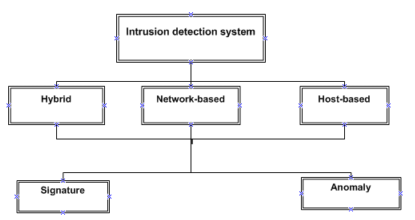
\includegraphics[width=0.5\textwidth]{idsBreakdown.png}
		\caption{A general breakdown of IDSs by Audit System and Event Analysis. Image taken from \cite{Alenezi2012}}
		\label{breakdown}
	\end{figure}
    % Will need some filler intro stuff here

    % In this intro, explicitely state that the following information came from [Mell, Peter @ EDPACS] 
    \subsection{Audit Systems}
    	This section will breakdown IDSs by their audit system, which describes the source of the data that they analyse for intrusions. There are three main types of audit systems: \emph{Host-Based}, \emph{Network-Based}, and \emph{Application-Based}.
    	\subsubsection{Host-Based}
    		Host-Based IDSs (HIDS) are characterised by having detection sensors on each individual machine within a network. These types of systems monitor an individual computer's system logs to detect attacks. HIDSs are able to detect attacks with much more specificity than network-based systems because they are able to monitor individual processes on an particular machine for malicious activity. 
    		
    		There are many advantages to using a HIDS. First, and fore most, they are able to detect attacks that network-based sensors cannot, because they are running on the host machine. Next, unlike network-based sensors, they are fully functional within both switched, and encrypted networks because their audit source is independent of network traffic, and they are able to use host resources to decrypt traffic before analysis.
    		
    		
    	\subsubsection{Network-Based}
    		Network-based IDSs (NIDS) are characterised by having detection sensors placed at network hubs, such as routers, rather than on each individual machine in a network. These types of systems work by monitoring network traffic looking for patterns in flow or analysing packet headers for trends. These are the most commonly used types of systems today. 
    		
    		NIDSs have many advantages over a host-based system, mainly that fewer sensors are required to cover the entire network, which also means less installation time and maintenance. These types of systems also have little to no impact on network performance, because they are sensors that traffic is simply routed through. As they are their own independent system residing on the network, they can be set up in such a way that they are invisible to outsiders. This hidden nature also makes them very insulated from attack themselves, which is a large advantage for network administrators. 
    		
    		However, these systems are not without their drawbacks. It has been shown that in periods of high network load, these systems performance drops due to an inability to process all incoming packets. As such, they could fail to detect an attack that was launched during one of these periods. The effectiveness of these types of systems also drops in switched networks, because switches subdivide network traffic such that a NIDS can no longer monitor all traffic on the network because much of it is hidden behind a switches. Finally, NIDSs are are unable to analyse encrypted traffic. This incapability is a major drawback, especially in this day in age, as more and more traffic is being moved to encrypted channels of communication. 		
    	\subsubsection{Application-Based}
    \subsection{Event Analysis}
    	This section will further subdivide and discuss IDSs by event analysis, which describes the method of detection used given a particular audit source of data. These detection methods fall into two major categories: \emph{Signature Detection} and \emph{Anomaly Detection}.   
	    \subsubsection{Signature Detection}
    	\subsubsection{Anomaly Detection}
    		Anomaly detecting systems work by constructing a system profile of "normal" behavior, and use that profile to then detect abnormal behavior. The idea is that attacks are a subset of abnormal behavior, which will allow these types of systems to detect them. Most of these systems use some complex statistical analysis to determine when activity differs from the system profile. The major draw to these types of systems is that, unlike signature detection methods, these systems can detect not only variations on known attacks, but completely novel attacks as well. The problem with this functionality is that it is predicated on having an effective system profile, which is by no means trivial to produce. They require extensive training sets to learn from, of which few exist. In practice, these types of systems produce large numbers of false positives that require manual inspection to effectively classify as an attack or not. For this reason, few existing systems use this type of detection. IDSs using this type of detection mechanism are more an an open area of research than production level systems. 
    		\begin{figure}[h!]
		\centering
		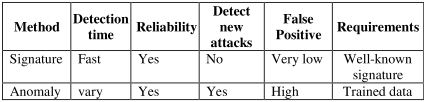
\includegraphics[width=0.5\textwidth]{signatreVSanomaly.png}
		\caption{Summary of Event Analysis systems. Image taken from \cite{Alenezi2012}}
		\label{comparison}
	\end{figure}
			

\section{Related Work}
    % I think we want to model this section after [Bhuyan, Bhattacharyya, Kalitan]
    % Their paper is in the probes section of Mendeley,you should go check it out
    \subsection{Probes}
    \subsection{Privilege Escalation}
    \subsection{Denial of Service}

\section{Methods}
    % This is where we should talk about why we broke attacks up the way that we 
    % did.

\section{Evaluation}
    % I am not so sure we even need this section, if we use it we could talk 
    % about the limitations of IDS's of something, the current state of affairs

\section{Discussion}
    % What would we say here?
    \subsection{Training Sets}
    \subsection{Effective Defense}
    \subsection{Open Problems}

\section{Conclusions}
    % See outline for this bit

	% References-------------------------------
	%I produced all references, we invariably wont use all of them, but this makes it easier to cite things trhoughout the paper. At the end, we will re-Export the bibTex, to just be what we used by searching through this document for the work 'cite'
	
% The following two commands are all you need in the
% initial runs of your .tex file to
% produce the bibliography for the citations in your paper.
\bibliographystyle{abbrv}
\bibliography{allSources}{}  % sigproc.bib is the name of the Bibliography in this case
\nocite{*}
% You must have a proper ".bib" file
%  and remember to run:
% latex bibtex latex latex
% to resolve all references
%
% ACM needs 'a single self-contained file'!
%
\balancecolumns
\end{document}
